
\section{Design}

To evaluate the workloads, we established a Kubernetes cluster with automated creation and teardown procedures using Terraform~\cite{terraform}, deployed on the Google Cloud Kubernetes Engine. We successfully deployed Koordinator \cite{koo} and Spark Operator on our cluster. The architecture overview is depicted in Fig. \ref{fig:arch}.

\begin{figure*}[h]
    \centering
    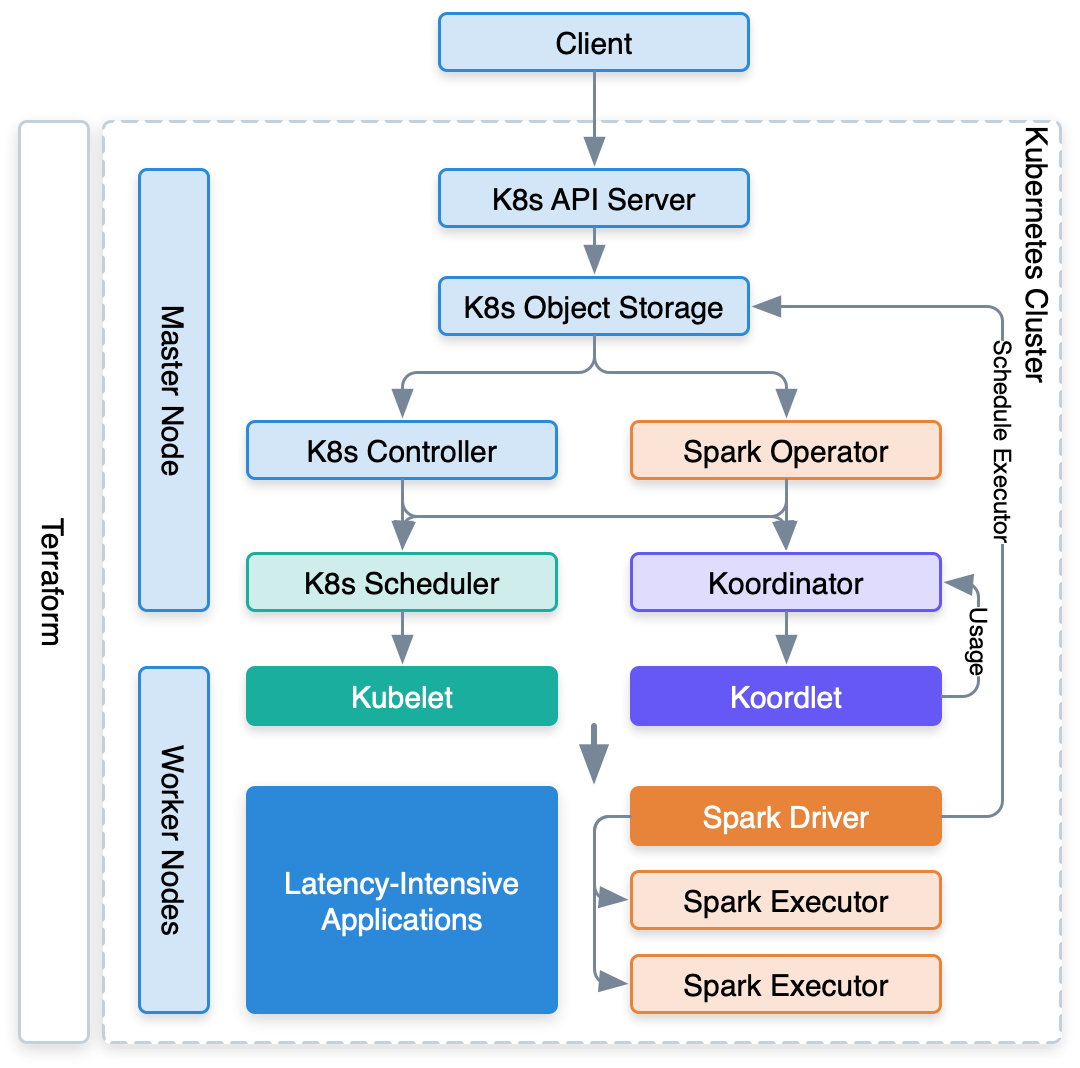
\includegraphics[width=0.7\textwidth]{img-arch.png}
    \caption{Architecture}
    \label{fig:arch}
\end{figure*}

\subsection{Control Plane}

Within the cluster, we configured Koordinator (scheduler, descheduler, controller manager) and Spark Operator. Both contain a Controller \cite{kcontroller} component responsible for synchronizing workload configuration from Kubernetes internal object storage (etcd) to the cluster. Koorinator also contains a scheduler which handles workload scheduling (through selectors), including Spark workloads.

Spark Operator listens to the desired state for Spark applications defined in etcd, delegating the actual scheduling to the assigned scheduler. After submiting a spark application configuration through Kubernets API, Spark Operator will try to tell scheduler to set up corresponding Spark Driver and Spark Executors for this application.

We set up two namespace for running experimental group and control group. For the experimental group, all workloads are scheduled by Koordinator scheduler.

For internal authorization, Spark Operator and Koordinator have the "editor" role for the entire cluster, simplifying testing procedures.

\subsection{Schedulers}

Alongside Kubernetes' default scheduler, Koordinator's scheduler operates independently as another option for workloads.

Kubernetes' default scheduler ensures every workload gets its requested resources, rejecting new workload requests when free resources are insufficient, and waiting until there is enough space for new workload. Through eviction policy we could force a new workload to be scheduled with the cost of killing other pods. In our setup, we disabled this behavior to avoid affecting existing workloads.

Koordinator's scheduler profiles real-time actual resource usage through Koordlet and aims to use the free space between requested resources and actual usage to maximize overall cluster resource usage. We set memory and CPU reclaim thresholds to 65\% for testing, leaving 35\% of CPU and memory requests un-colocatable for other workloads as a headroom for spikes.

\subsection{Workloads}

Two workload types were tested: applications and batch jobs.

Application workload was simulated using looksbusy \cite{looksbusy} as a single pod with varying CPU and memory requests on host nodes.

For batch jobs, we used two examples provided by Spark to simulate simple/short batch jobs (using SparkPI \cite{sparkexamples}) and intense batch jobs (using SparkTC \cite{sparkexamples}).

Spark workloads were used to test Koordinator's over-commitment capabilities. In this scenario, pods occupy the cluster requesting more resources than needed. This stable stress setup demonstrates the benefits of utilizing Koordinator's over-commitment feature. With insufficient allocatable resources, overall CPU utilization remains low, providing room for Koordinator to co-locate jobs and improve resource utilization.
